\documentclass{article}
\usepackage{blindtext}
\usepackage{geometry}
\usepackage{multicol}
\usepackage{amsmath}
\usepackage{graphicx}
\usepackage[dvipsnames]{xcolor}
\usepackage{lipsum}
\usepackage{amssymb}
\usepackage{tikz}
\usepackage{ntheorem}
\usepackage{mdframed}
\usepackage{float}
\usepackage{color}
\usepackage[shortlabels]{enumitem}

\usepackage{import}
\usepackage{xifthen}
\usepackage{pdfpages}
\usepackage{transparent}

\pdfsuppresswarningpagegroup=1

\geometry{ a4paper, total={170mm,257mm},
	left=20mm, top=20mm, }

\theoremseparator{}
\newmdtheoremenv[
	skipabove=10pt,
	skipbelow=10pt,
	linecolor=black,
	backgroundcolor=gray!10,
	roundcorner=5pt,
]{frm-ex}{Example}

\theoremseparator{}
\newmdtheoremenv[
	skipabove=10pt,
	skipbelow=10pt,
	linecolor=black,
	backgroundcolor=gray!10,
	roundcorner=5pt,
]{frm-prf}{Proof}

\newcommand{\SubItem}[1]{
	{\setlength\itemindent{15pt} \item[-] #1}
}

\newenvironment{rcases}
{\left.\begin{aligned}}
		{\end{aligned}\right\rbrace}

\newcommand{\mathbbD}{\mathbb{D}}
\newcommand{\mathbbR}{\mathbb{R}}

\begin{document}
%\begin{multicols*}{2}
\section{Important Definitions}
\subsection{Norm}
The norm $|x|$ of a vector $x$ is a real valued function with the following properties:
\begin{enumerate}[label=(\roman*)]
	\item $|x| \geq 0$ with $|x|=0$ if and only if $x=0$
	\item $|\alpha x|=|\alpha| x \mid$ for any scalar $\alpha$
	\item $|x+y| \leq|x|+|y|$ (triangle inequality)
\end{enumerate}
The norm $|x|$ of a vector $x$ can be thought of as the size or length of the vector $x$. Similarly, $|x-y|$ can be thought of as the distance between the vectors $x$ and $y$.
\subsection{Induced Norm}
Let $|\cdot|$ be a given vector norm. Then for each matrix $A \in \mathcal{R}^{m \times n}$, the quantity $\|A\|$ defined by
\(
\|A\| \triangleq \sup _{\substack{x \neq 0 \\ x \in \mathcal{R}^n}} \frac{|A x|}{|x|}=\sup _{|x| \leq 1}|A x|=\sup _{|x|=1}|A x|
\)
is called the induced (matrix) norm of $A$ corresponding to the vector norm $|\cdot|$.
\\\\
Some of the properties of the induced norm that we will often use in this book are summarized as follows:
\begin{enumerate}[label=(\roman*)]
	\item $|A x| \leq\|A\||x|, \quad \forall x \in \mathcal{R}^n$
	\item $\|A+B\| \leq\|A\|+\|B\|$
	\item $\|A B\| \leq\|A\|\|B\|$
\end{enumerate}
\subsection{$\mathcal{L}_p$ spaces}
for functions fo time, we define the $\mathcal{L}_p$ norm
\begin{equation*}
	\|x\|_p \triangleq\left(\int_0^{\infty}|x(\tau)|^p d \tau\right)^{1 / p}
\end{equation*}
for $p \in[1, \infty)$ and say that $x \in \mathcal{L}_p$ when $\|x\|_p$ exists (i.e., when $\|x\|_p$ is finite). The $\mathcal{L}_{\infty}$ norm is defined as
$$
	\|x\|_{\infty} \triangleq \sup _{t \geq 0}|x(t)|
$$
and we say that $x \in \mathcal{L}_{\infty}$ when $\|x\|_{\infty}$ exists.
In the above $\mathcal{L}_p, \mathcal{L}_{\infty}$ norm definitions, $x(t)$ can be a scalar or a vector function. If $x$ is a scalar function, then $|\cdot|$ denotes the absolute value. If $x$ is a vector function in $\mathcal{R}^n$ then $|\cdot|$ denotes any norm in $\mathcal{R}^n$.
\begin{frm-ex}[$\mathcal{L}_p$ spaces]
Consider the function $f(t)=\frac{1}{1+t}$. Then,
$$
	\begin{gathered}
		\|f\|_{\infty}=\sup _{t \geq 0}\left|\frac{1}{1+t}\right|=1, \quad\|f\|_2=1
	\end{gathered}
$$
Hence, $f \in \mathcal{L}_2 \bigcap \mathcal{L}_{\infty}$ but $f \notin \mathcal{L}_1 ; f$, however, belongs to $\mathcal{L}_{1 e}$, i.e., for any finite $t \geq 0$, we have
$$
	\int_0^t \frac{1}{1+\tau} d \tau=\ln (1+t)<\infty
$$
\end{frm-ex}
\begin{itemize}
	\item A function $f$ belongs to $\mathcal{L}_1$ if the integral of the absolute value of $f$ over its entire domain is finite. Mathematically, this can be expressed as:
	      \[ \int |f(x)| \, dx < \infty \]
	      In $\mathcal{L}_1$, functions are required to have a finite "$\mathcal{L}_1$  norm."
	\item  A function $f$ belongs to $\mathcal{L}_2$ if the square of the absolute value of $f$ is Lebesgue integrable, meaning:
	      \[ \int |f(x)|^2 \, dx < \infty \]
	      In $\mathcal{L}_2$, functions are required to have a finite "L norm."
	\item A function $f$ belongs to $\mathcal{L}_\infty$ if it is bounded, meaning there exists a constant $M$ such that $|f(x)| \leq M$ for all $x$. In $\mathcal{L}_\infty$, functions are required to have a finite "norm," which is essentially the supremum (maximum) of the absolute value of the function.
\end{itemize}
\section{Fundamental Properties}
\subsection{Existence and Uniqueness}
\subsubsection{Local Existence and Uniqueness}
Let $f(t,x)$ be piecewise continuous in $t$ and satisfy the Lipschitz condition
\begin{equation*}
	||f(t,x)-f(t,y)||\leq L ||x-y||
\end{equation*}
$\forall x,y \in B = \{x \in \mathbb{R}^n\; | \; ||x-x_0|| \leq r\}, \; \forall t \in [t_0,t_1]$. Then, there exists some $\delta > 0$ such that the state equation $\dot x = f(t,x)$ with $x(t_0)=x_0$ has a unique solution over $[t_0,t_0+\delta]$.
\subsubsection{Lipschitz Condition}
Let $f \: : \: [a,b] \times D \rightarrow R^m$ be continuous or some domain $D
	\subset R^n$. Suppose that $[\partial f / \partial x]$ exists and is continuous
on $[a,b] \times D$. If, for a convex subset $W \subset D$, there is a constant
$L \geq 0$ such that
\begin{equation*}
	\left|\left|\frac{\partial f}{\partial x}(t,x)\right|\right| \leq L
\end{equation*}
on $[a,b] \times W$, then
\begin{equation*}
	||f(t,x) - f(t,y)|| \leq L||x-y||
\end{equation*}
for all $t \in [a,b], \: x \in W$, and $y \in W$.
\subsubsection{Locally Lipschitz}
If $f(t,x)$ and $[\partial f / \partial x](t,x)$ are continuous on $[a,b]
	\times D$, for some domain $D \subset R^n$, then $f$ locally Lipschitz in $x$
on $[a,b] \times D$.
\subsubsection{Globally Lipschitz}
If $f(t,x)$ and $[\partial f / \partial x](t,x)$ are continuous on $[a,b]
	\times R^n$, then $f$ is globally Lipschitz in $x$ on $[a,b] \times R^n$ if and
only if $[\partial f / \partial x]$ is uniformly bounded on $[a,b] \times R^n$
\subsubsection{Global Existence and Uniqueness}
Suppose that $f(t,x)$ is piecewise continuous in $t$ and satisfies
\begin{equation*}
	||f(t,x)-f(t,y)|| \leq L||x-y||
\end{equation*}
$\forall x,y \mathbb{R}^n,\forall t \in [t_0,t_1]$. Then, the state equation $\dot x = f(t,x)$, with $x(t_0)=x_0$, has a unique solution over $[t_0,t_1]$.
\subsubsection{Existence and Uniqueness Theorem}
\newpage
\section{Second-Order Systems}
\subsection{Limit Cycles}
We consider a two-dimensional dynamical system of the form
\begin{equation*}
	\dot x(t) = V(x(t))
\end{equation*}
where $V: \mathbb{R}^2 \to \mathbb{R}^2$ is a smooth function. A trajectory of this system is some smooth function $x(t)$ with values in $\mathbb{R}^2$ which satisfies this differential equation. Such a trajectory is called closed (or periodic) if it is not constant but returns to its starting point, i.e., if there exists some $t_0 > 0$ such that $x(t + t_0) = x(t)$ for all $t \in \mathbb{R}$. An orbit is the image of a trajectory, a subset of $\mathbb{R}^2$. A closed orbit, or cycle, is the image of a closed trajectory. A limit cycle is a cycle which is the limit set of some other trajectory.
\begin{figure}[H]
	\centering
	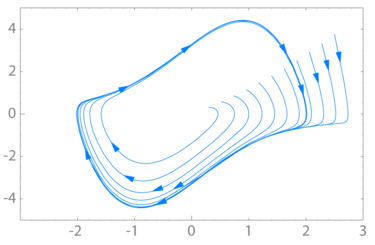
\includegraphics[width = 0.4\textwidth]{figures/375px-VanDerPolPhaseSpace.png}
	\caption{Stable Limit Cycle}
\end{figure}
\subsubsection{Poincaré-Bendixson Criterion}
Consider the system \(\dot x = f(x)\) and let $M$ be a closed bounded subset of
the plane such that
\begin{itemize}
	\item $M$ contains no equilibrium points or contains only one equilibrium point such that the Jacobian matrix $[\partial f / \partial x]$ at this point has eigenvalues with positive real parts. (Hence, the equilibrium point is unstable focus or unstable node.)
	\item  Every trajectory starting in $M$ stays in $M$ for all future time.
\end{itemize}
Then, $M$ contains a periodic orbit of $\dot x = f(x)$.
\subsubsection{Benixson Criterion}
If, on a simply connected region ($\mathcal{C}^1$) $D$ of the plane, the
expression $\partial f_1 / \partial x_1 + \partial f_2 / \partial x_2$ is not
identically zero and does not change sign, then $\dot x= f(x)$ has no periodic
orbits lying entirely in D. \newpage
\section{Lyapunov Stability}
\subsection{Autonomous Systems}
\subsubsection{Stability Principles}
The equilibrium point $x=0$ of $\dot x = f(X)$ is
\begin{itemize}
	\item stable if, for each $\epsilon > 0$, there is a $\delta = \delta(\epsilon) > 0$
	      such that
	      \begin{equation*}
		      ||x(0)|| < \delta \Rightarrow ||x(t)|| < \epsilon, \quad \forall t \geq 0
	      \end{equation*}
	\item unstable if it is not stable
	\item asymptotically stable if it is stable and $\delta$ can be chosen such that
	      \begin{equation*}
		      ||x(0)|| < \delta \Rightarrow \lim_{t\rightarrow \infty} \; x(t) = 0
	      \end{equation*}
\end{itemize}
\subsubsection{Quadratic Lyapunov Function}
\begin{equation}
	V(x) = \frac{1}{2}x^T Px \textrm{ , } P > 0
\end{equation}
and
\begin{equation}
	\begin{split}
		\frac{d}{dt}V(x) & = \frac{1}{2} x^T P Ax + (x^T PAx)^T \\
		                 & = \frac{1}{2} 2 x^T P\dot x          \\
		                 & = x^T P\dot x
	\end{split}
\end{equation}
\begin{equation}
	\dot V(x) = x^T P\dot x
\end{equation}
In other words
\begin{equation}
	\dot V(x) =
	\begin{bmatrix}
		x_1 \\
		x_2
	\end{bmatrix}^T
	\begin{bmatrix}
		p_{11} & p_{21} \\
		p_{12} & p_{22}
	\end{bmatrix}
	\begin{bmatrix}
		\dot x_1 \\
		\dot x_2
	\end{bmatrix}
\end{equation}
\subsubsection{Asymptotically Stable}
Let $x = 0$ be an equilibrium point and $D \subset R^n$ be a domain containing
$x = 0$. Let $V\::\:D \rightarrow R$ be a continuously differentiable function
such that
\begin{equation}
	V(0) = 0 \quad \textrm{and} \quad V(x) > 0 \; \textrm{in} \; D - \{0\}
\end{equation}
\begin{equation}
	\dot{V}(x) \leq 0 \; \textrm{in} \; D
\end{equation}
Then $x=0$ is stable. Moreover, if
\begin{equation}
	\dot{V}(x) < 0 \; \textrm{in} \; D - \{0\}
\end{equation}
then $x=0$ is asymptotically stable.
\subsubsection{Globally Asymptotic stable}
Let $x=0$ be an equilibrium point or $\dot x = f(x)$. Let $V : \mathbb{R}^n
	\rightarrow \mathbb{R}$ be a continuously differentiable function such that
\begin{equation*}
	V(0) = 0 \text{  and  } V(x) > 0, \; \forall x \neq 0
\end{equation*}
\begin{equation*}
	||x|| \rightarrow \infty \Rightarrow V(x) \rightarrow \infty
\end{equation*}
\subsubsection{Radially Unbounded Function}
A radially unbounded function is a function $f : \mathbb{R}^n \rightarrow
	\mathbb{R}$ for which
\begin{equation*}
	||x|| \rightarrow \infty \Rightarrow f(x) \rightarrow \infty
\end{equation*}
Or equivalently
\begin{equation*}
	\forall c > 0 : \exists r > 0 : \forall x \in \mathbb{R}^n : [||x|| > r \Rightarrow f(x) > c]
\end{equation*}
\subsubsection{Region of attraction}
The region of attraction is also called the region of asymptotic stability. The
region of attraction may be hard to calculate exactly, but Lyapunov functions
can be used to estimate this region. \\\\ First of all, the region of
attraction must satisfy the following: from the definition of asymptotic
stability we see that if there is a Lyapunov function that satisfy the
condition of asymptotic stability over a domain $\mathbb{D}$ and if $\Omega_c =
	\{ x \in \mathbb{R}^n | V(x) \leq c\}$ is bounded and contained in $\mathbbD$,
then ecery trajectory starting in $\Omega_c$ remains in $\Omega_c$ and
approaches the origin as $t \to \infty$ \\\\ Let $x=0$ be an asymptotically
stable equilibrium point of the system $\dot x = f(x)$, where $f : \mathbb{D}
	\to \mathbb{R}^n$ is locally lipschitz and $\mathbb{D} \subset \mathbb{R}^n$ is
a domain that contains the origin. Let $t \to \phi(t;x_0)$ be the solution of
$\dot x = f(x)$ that starts at initial state $x_0$ at time $t=0$. The region of
attraction of the origin, denoted by $R_A$, is defined by
\begin{equation*}
	R_A = \{ x_0 \in \mathbb{D} : \phi(t;x_0) \text{ is defined }\forall t \geq 0 \text{ and } \phi(t;x_0) \to \text{ as } t \to \infty \}
\end{equation*}
I.e. the region of attraction $R_A$ is the set of all points $x_0$ in $\mathbb{D}$ such that the solution of
\begin{equation*}
	\dot x = f(x) \qquad x(0) = x_0
\end{equation*}
is defined for all $t \geq 0$ and converges to the origin as $t \to \infty$.
\begin{frm-ex}[Example of region of attraction]
\item
Our domain $\mathbbD$ is defined as
\begin{equation*}
	\mathbbD = \{ x \in \mathbbR^2 : x_1 + x_2 < 1\}
\end{equation*}
where $\dot V(x) < 0$. Our region of attraction is defined as
\begin{equation*}
	\Omega_c = \{ x \in \mathbbR^2 : V(x) \leq c \}
\end{equation*}
where $c < \min(V(x)$ and $x \in \partial c$ (x is on the border of $c$).
\begin{equation*}
	\begin{split}
		x_1 + x_2 & = 1       \\
		x_1       & = 1 - x_2
	\end{split}
\end{equation*}
Then we minimize $V(x)$ with respect of $x_2$
\begin{equation*}
	\begin{split}
		\min(V(x))_{x_2}\bigg|_{x_1=1-x_2} & = min_{x_2}(\frac{1}{2}((1-x_2)^2+x_2^2)) = 0               \\
		\min_{x_2}(\frac{1}{2}-x_2+x_2^2)  & = \frac{\partial}{\partial x_2} (\frac{1}{2}-x_2+x_2^2) = 0 \\
		-1 + x_2                           & = 0                                                         \\
		x_2                                & = \frac{1}{2} \quad \to \quad x_1 = \frac{1}{2}
	\end{split}
\end{equation*}
Further, we must satisfy $c < V(\frac{1}{2}, \frac{1}{2}) = \frac{1}{4}$. We have therefore the following region of attraction
\begin{equation*}
	\Omega_{\frac{1}{4}} = \{x \in \mathbbR^2 : V(x) \leq \frac{1}{4}\}
\end{equation*}
\end{frm-ex}
\subsection{The Invariance Principle}
\subsubsection{Invariant Set}
A set $M$ is said to be an invariant set with respect to $\dot x = f(x)$ iff
\begin{equation*}
	x(0) \in M \quad \Rightarrow \quad x(t) \in M, \qquad \forall t \in \mathbb{R}
\end{equation*}
\subsubsection{Positively Invariant Set}
A set $M$ is a positively invariant set with respect to $\dot x = f(x)$ iff
\begin{equation*}
	x(0) \in M \quad \Rightarrow \quad x(t) \in M, \qquad \forall t \geq 0
\end{equation*}
\subsubsection{Lasalle's Theorem}
Lasalle's invariance principle can be used to show the asymptotic stability of
an equilibrium point when $\dot V$ is negative semi-definite, $i.e \quad \dot V
	\leq 0$. $\dot V$ is semidefinite if $\dot V$ is not sticly 0 in origo. \\\\
Let $\Omega \subset D$ be a compact set that is positively invariant with
respect to $\dot x = f(x)$. Let $V\::\:D \rightarrow R$ be a continuously
differentiable function such that $\dot V(x) \leq 0$ in $\Omega$. Let $E$ be
the set of all points in $\Omega$ where $\dot V(x) = 0$. Let $M$ be the largest
invariant set in E. Then every solution starting in $\Omega$ approaches $M$ as
$t \rightarrow \infty$.
\begin{figure}[h]
	\centering
	\def\svgwidth{0.5\columnwidth}
	\input{figures/Lasalles.eps_tex}
\end{figure}
\subsubsection{Barbashin Theorem}
Let $x=0$ be an equilibrium point for \[\dot{x} = f(x)\]
Let $V: D \rightarrow R$ be a continuously differentiable positive definite
function on a domain $D$ containing the origin $x=0$, such that $\dot V(x) \leq
	0$ in $D$. Let $S=\{x \in D\:|\:\dot V(x) = 0\}$ and suppose that no solution
can stay identically in $S$, other than the trivial solution $x(t) \equiv 0$.
Then, the origin is asymptotically stable. If a $A$ matrix i Hurwitz, we can
conclude asymptotic stability.
\subsubsection{Krasovskii Theorem}
Let \(x = 0\) be an equilibrium point for the system\[\dot{x} = f(x)\]. Let \(V : \mathbb{R}^n \to \mathbb{R}\) be a continuously differentiable, radially unbounded, positive definite function such that \(V(x) \leq 0\) for all \(x \in \mathbb{R}^n\). Let \(S = \{x \in \mathbb{R}^n \,|\, V(x) = 0\}\) and suppose that no solution can stay identically in \(S\), other than the trivial solution \(x(t) = 0\). Then, the origin is globally asymptotically stable.
\subsubsection{Dominating cross-terms}
\paragraph{Completion of squares}
\begin{equation*}
	x_1x_2 \leq \frac{1}{2}(x_1^2 + x_2^2) = \frac{1}{2} ||x||^2_2
\end{equation*}
Another alternative is to write $\dot V$ as $-x^TQx$, where $Q=Q^T$ is positive definite
\paragraph{Youngs inequality}
\begin{equation*}
	xy \leq \epsilon x^2 + \frac{1}{4\epsilon}y^2, \quad \forall \epsilon > 0 \; \forall x,y \in \mathbb{R}
\end{equation*}
\subsubsection{Handling terms with indeterminate sign}
\paragraph{Cauchy-Schwarz Inequality}
\begin{equation*}
	|a_1x_1+a_2x_2+...+a_nx_n|\leq\sqrt{(a_1^2+a_2^2+...+a_n^2}||x||_2
\end{equation*}
\subsection{Linear Systems and Linearization}
\subsubsection{Hurwitz matrix / Stability matrix}
$A$ matrix $A$ is Hurwitz; that is, $Re\{\lambda_i\} < 0$ for all eigenvalues of $A$, if
and only if for any given positive definite symmetric matrix $Q$ there exists a positive
definite symmetric matrix $P$ that satisfies the \textit{Lyapunov equation (\ref{Lyapunov 4.12})}. Moreover,
if $A$ is Hurwitz, then P is the unique solution of (\ref{Lyapunov 4.12}).
\begin{equation}
	PA+A^TP=-Q
	\label{Lyapunov 4.12}
\end{equation}
\\
Another way one can prove asymptotic stability in the origin is by using this symmetric matrix $Q$. We can write $\dot V(x)$ as the following
\begin{equation*}
	\dot V(x) = x^T P \dot x + \dot x^T P x = -x^T Q x
\end{equation*}
If $Q$ is positive definite, we can conclude asymptotic stability at the origin.
\\
\begin{frm-ex}[Example using Hurwitz matrix]
\item
We have the following $\dot V(x)$
\begin{equation*}
	\dot V(x) \leq -x_2^2\left(2 - \frac{1}{4\epsilon}\right) - x_1x_2 - x_1^2(1-\epsilon)
\end{equation*}
We can then formulate the following $Q$ matrix
\begin{equation*}
	Q =
	\begin{bmatrix}
		1 - \epsilon & \frac{1}{2}              \\
		\frac{1}{2}  & 2 - \frac{1}{4 \epsilon}
	\end{bmatrix}
\end{equation*}
To ensure that $Q$ is positive definite we can evaluate the principle of minors
\begin{equation*}
	(1 - \epsilon) \left( w - \frac{1}{4 \epsilon} \right) - \frac{1}{4} > 0
\end{equation*}
while $(1 - \epsilon) > 0$. We can solve the las inequality, and $\epsilon$ must satisfy
\begin{equation*}
	\frac{2 - \sqrt{2}}{4} < \epsilon < \frac{2 + \sqrt{2}}{4}
\end{equation*}
to ensure that the origin is asymptotically stable.
\end{frm-ex}

\subsubsection{Indirect Method}
Let \(x = 0\) be an equilibrium point for the nonlinear system
\[
	\dot{x} = f(x)
\]
where \(f : D \to \mathbb{R}^n\) is continuously differentiable and \(D\) is a
neighborhood of the origin. Let
\[
	A = \frac{\partial f}{\partial x_i}\bigg|_{x=0}
\]
Then,
\begin{enumerate}
	\item The origin is asymptotically stable if \(\text{Re}(\lambda_i) < 0\) for all
	      eigenvalues \(\lambda_i\) of \(A\).
	\item The origin is unstable if \(\text{Re}(\lambda_i) > 0\) for one or more of the
	      eigenvalues \(\lambda_i\) of \(A\).
\end{enumerate}
\subsection{Comparison Functions}
\subsubsection{Class $\mathcal{K}$ and Class $\mathcal{K}_{\infty}$ Definitions}
A continuous function \(\alpha : [0, a) \to [0, \infty)\) is said to belong to class \(\mathcal{K}\) if it is strictly increasing and \(\alpha(0) = 0\). It is said to belong to class \(\mathcal{K}_\infty\) if \(a = \infty\) and \(\alpha(r) \to \infty\) as \(r \to \infty\).
\subsubsection{Class $\mathcal{K}\mathcal{L}$ Definition}
A continuous function \(\beta : [0, a) \times [0, \infty) \to [0, \infty)\) is said to belong to class \(\mathcal{K}\mathcal{L}\) if, for each fixed $s$, the mapping $\beta(r,s)$ belongs to $\mathcal{K}$ with respect to $r$ and, for each fixed $r$, the mapping $\beta(r,s)$ is decreasing with respect to $s$ and \(\beta(r,s) \to \infty\) as \(s \to \infty\).
%\end{multicols*}
\subsubsection{Class $\mathcal{K}$, $\mathcal{K}_{\infty}$ and $\mathcal{K}\mathcal{L}$ Rules}
Let $\alpha_1$ and $\alpha_2$ be class $\mathcal{K}$ functions on $[0,a),\alpha_3$ and $\alpha_4$ be class $\mathcal{K}-\infty$
\begin{frm-ex}[Class $\mathcal{K}$]

\item $\alpha(r) = \tan^{-1}$ is strictly increasing since $\dot \alpha(r)=\frac{1}{(1+r^2)}>0$. It belongs to calss $\mathcal{K}$, but not to class $\mathcal{K}_{\infty}$ since $\lim_{r \rightarrow \infty} \alpha(r) = \frac{\pi}{2} < \infty$.
\end{frm-ex}
\begin{frm-ex}[Class $\mathcal{K}\mathcal{L}$]
\item $\beta(r,s) = \frac{r}{(ksr+1)}$ , for any positive real number $k$, is strictly increasing in $r$ since
\begin{equation*}
	\frac{\partial \beta}{\partial r} = \frac{ks}{(ksr+1)^2} > 0
\end{equation*}
and stricly decreasuing in $s$ since
\begin{equation*}
	\frac{\partial \beta}{\partial s} = \frac{-kr^2}{(ksr+1)^2} < 0
\end{equation*}
Moreover $\beta(r,s) \rightarrow 0 \text{ as } s \rightarrow \infty$
\end{frm-ex}
\subsubsection{Introducing class $\mathcal{K}$ functions in Lyapunov's stability theorem}
Let $\alpha_1$ and $\alpha_2$ be class $\mathcal{K}$ functions on $[0, a), \alpha_3$ and $\alpha_4$ be class $\mathcal{K}_{\infty}$ functions, and $\beta$ be a class $\mathcal{K} \mathcal{L}$ function. Denote the inverse of $\alpha_i$ by $\alpha_i^{-1}$. Then,
\begin{itemize}
	\item $\alpha_1^{-1}$ is defined on $\left[0, \alpha_1(a)\right)$ and belongs to class $\mathcal{K}$.
	\item $\alpha_3^{-1}$ is defined on $[0, \infty)$ and belongs to class $\mathcal{K}_{\infty}$.
	\item $\alpha_1 \circ \alpha_2$ belongs to class $\mathcal{K}$.
	\item $\alpha_3 \circ \alpha_4$ belongs to class $\mathcal{K}_{\infty}$.
	\item $\sigma(r, s)=\alpha_1\left(\beta\left(\alpha_2(r), s\right)\right)$ belongs to class $\mathcal{K} \mathcal{L}$.
\end{itemize}
Class $\mathcal{K}$ and class $\mathcal{K} \mathcal{L}$ functions enter into Lyapunov analysis through the next subsections
\subsubsection{Lyapanovs analysis with Class $\mathcal{K}$ functions}
Let $V: D \rightarrow R$ be a continuous positive definite function defined on a domain $D \subset R^n$ that contains the origin. Let $B_r \subset D$ for some $r>0$. Then, there exist class $\mathcal{K}$ functions $\alpha_1$ and $\alpha_2$, defined on $[0, r]$, such that
\[
	\alpha_1(\|x\|) \leq V(x) \leq \alpha_2(\|x\|)
\]
for all $x \in B_r$. If $D=R^n$, the functions $\alpha_1$ and $\alpha_2$ will
be defined on $[0, \infty)$ and the foregoing inequality will hold for all $x
	\in R^n$. Moreover, if $V(x)$ is radially unbounded, then $\alpha_1$ and
$\alpha_2$ can be chosen to belong to class $\mathcal{K}_{\infty}$.
\subsubsection{Lyapanovs analysis with Class $\mathcal{K} \mathcal{L}$ functions}
Consider the scalar autonomous differential equation
$$
	\dot{y}=-\alpha(y), \quad y\left(t_0\right)=y_0
$$
where $\alpha$ is a locally Lipschitz class $\mathcal{K}$ function defined on $[0, a)$. For all $0 \leq y_0<a$, this equation has a unique solution $y(t)$ defined for all $t \geq t_0$. Moreover,
$$
	y(t)=\sigma\left(y_0, t-t_0\right)
$$
where $\sigma$ is a class $\mathcal{K} \mathcal{L}$ function defined on $[0, a) \times[0, \infty)$.
\subsection{Nonautonomous Systems}
Throughout this section we will consider the following Nonautonomous system
\begin{equation*}
	\dot x = f(t,x)
	\label{Nonautonomous system}
\end{equation*}
\subsubsection{Uniformity}
Proving uniformity means that the initial condition $x_0$ has no effect on the stability of the system.

Uniformity $\mapsto$ convergence rate not dependent on $t_0$.

\subsubsection{Stability definitions}
The equilibrium point $x=0$ of \ref{Nonautonomous system} is
\begin{itemize}
	\item stable if, for each $\varepsilon>0$, there is $\delta=\delta\left(\varepsilon,
		      t_0\right)>0$ such that $$ \left\|x\left(t_0\right)\right\|<\delta
		      \Rightarrow\|x(t)\|<\varepsilon, \quad \forall t \geq t_0 \geq 0 $$
	\item uniformly stable if, for each $\varepsilon>0$, there is
	      $\delta=\delta(\varepsilon)>0$, independent of $t_0$, such that (4.16) is
	      satisfied.
	\item unstable if it is not stable.
	\item asymptotically stable if it is stable and there is a positive constant
	      $c=c\left(t_0\right)$ such that $x(t) \rightarrow 0$ as $t \rightarrow \infty$,
	      for all $\left\|x\left(t_0\right)\right\|<c$.
	\item Asymptotically stable (AS) if \subitem it is stable \subitem there exists $c>0$
	      s.t. for all $t_0 \geq 0$ and $\eta>0$, there exists $T\left(t_0,
		      \eta\right)>0$ satisfying $$ \left\|x\left(t_0\right)\right\| \leq c
		      \Longrightarrow\|x(t)\| \leq \eta \quad \forall t \geq t_0+T\left(t_0,
		      \eta\right) $$
	\item Uniformly asymptotically stable (UAS) if \subitem it is uniformly stable (US)
	      \subitem there exists $c>0$ s.t. for all $t_0 \geq 0$ and $\eta>0$, there
	      exists $T(\eta)>0$ satisfying $$ \left\|x\left(t_0\right)\right\| \leq c
		      \Longrightarrow\|x(t)\| \leq \eta \quad \forall t \geq t_0+T(\eta) $$

	\item Globally uniformly asymptotically stable (GUAS) if \subitem it is globally
	      uniformly stable (GUS) \subitem for all $\eta, c>0$ and $t_0 \geq 0$ there
	      exists $T(\eta, c)>0$ s.t. $$ \left\|x\left(t_0\right)\right\| \leq c
		      \Longrightarrow\|x(t)\| \leq \eta \quad \forall t \geq t_0+T(\eta, c) $$
\end{itemize}
\subsubsection{Equlibirum Points}
$x^* \in \mathbb{R}^n$ is an equilibrium point of $\dot x = f(t,x)$ if $f(t,x^*) = 0$ for all $t \geq 0$.
\begin{frm-ex}[Example of equilibrium point]
\item $\dot x = -\frac{a(t)x}{1+x^2}$ has the equilibrium point $x^* = 0$. We can see this by evaluating $f(t,x^*)$
\item $\dot x = -\frac{a(t)}{1+x^2}+b(t)$ where $b(t) \neq 0 \; \forall t$ has no equilibrium points
\end{frm-ex}
\subsubsection{Stability definitions with $\mathcal{K}$ and $\mathcal{KL}$ classes}
For $\dot x = f(t,x)$, the equilibrium point $x^* = 0$ is
\begin{itemize}
	\item Uniformly stable (US) if $\exists \alpha \in \mathcal{K}, \exists c > 0$ such
	      theoremseparator
	      \begin{equation*}
		      \| x(t) \| \leq \alpha(\|x(t_0\|)) \quad \forall t \geq t_0, \quad \|x(t_0)\| \leq c, \quad \forall t_0 \geq 0
	      \end{equation*}
	\item globally uniformly stable (GUS) if $\exists \alpha \in \mathcal{K}_{\infty}$
	      such that
	      \begin{equation*}
		      \| x(t) \| \leq \alpha(\|x(t_0\|)) \quad \forall t \geq t_0, \quad \forall t_0 \geq 0
	      \end{equation*}
	\item exponentially stable if $\exists c,k, \lambda > 0$
	      \begin{equation*}
		      \|x(t)\| \leq k \|x(t_0)\|e^{-\lambda(t-t_0)} \qquad t \geq t_0 \geq 0, qquad \|x(t_0)\| < c
	      \end{equation*}
	\item globally exponentially stable if $\exists k, \lambda > 0$
	      \begin{equation*}
		      \|x(t)\| \leq k \|x(t_0)\|e^{-\lambda(t-t_0)} \qquad t \geq t_0 \geq 0, qquad \forall x(t_0)
	      \end{equation*}
\end{itemize}
\subsubsection{Time-varying Lyapunov function candidates}
$V(t,x)$ is positive definite if
\begin{equation*}
	\begin{rcases}
		V(t,0) = 0 \\
		V(t,x) \geq W_1(x)
	\end{rcases}
	\forall t \geq 0 \text{, for some positive definitie function } W_1(x)
\end{equation*}
and
\begin{itemize}
	\item $(t,x) \rightarrow V(t,x)$ is positive semidefinite if $x \rightarrow	W_1(x)$ positive semidefinite
	\item $(t,x) \rightarrow V(t,x)$ is radially unbounded if $x \rightarrow	W_1(x)$ radially unbounded
\end{itemize}
$V(t,x)$ is decresent if
\begin{equation*}
	\begin{rcases}
		V(t,0) = 0 \\
		V(t,x) \leq W_2(x)
	\end{rcases}
	\forall t \geq 0, \text{ for some positive definite function } W_2(x)
\end{equation*}
\begin{figure}[h]
	\centering
	\input{figures/Lyapunov_functions.eps_tex}
\end{figure}
\subsubsection{Lyapunov theorem: Uniformal Stability}
If there exitst a function $V(t,x):[0, \infty) \times \mathbbD \rightarrow
	\mathbbR$ and $W_i: \mathbb{D} \rightarrow \mathbb{R}$ continuous positive
definite such that
\begin{enumerate}[i)]
	\item $V \text{ is } C^1$
	\item $W_1(x) \leq V(t,x) \leq W_2(x) \qquad \forall (t,x) \in [0, \infty) \times \mathbb{D}$
	\item $\dot V(t,x) \leq 0 \qquad \forall (t,x) \in [0, \infty) \times \mathbb{D}$
\end{enumerate}
then $x=0$ is uniformly stable.
\begin{figure}[h]
	\centering
	\resizebox{0.45\textwidth}{!}{\input{figures/Lyapunov_analysis.pdf_tex}}
\end{figure}
\begin{frm-prf}
The derivative of $V$ along the trajectories of (4.15) is given by
$$
	\dot{V}(t, x)=\frac{\partial V}{\partial t}+\frac{\partial V}{\partial x} f(t, x) \leq 0
$$
Choose $r>0$ and $c>0$ such that $B_r \subset D$ and $c<\min _{\|x\|=r}
	W_1(x)$. Then, $\left\{x \in B_r \mid W_1(x) \leq c\right\}$ is in the interior
of $B_r$. Define a time-dependent set $\Omega_{t, c}$ by $$ \Omega_{t,
		c}=\left\{x \in B_r \mid V(t, x) \leq c\right\} $$

The set $\Omega_{t, c}$ contains $\left\{x \in B_r \mid W_2(x) \leq c\right\}$
since $$ W_2(x) \leq c \Rightarrow V(t, x) \leq c $$

On the other hand, $\Omega_{t, c}$ is a subset of $\left\{x \in B_r \mid W_1(x)
	\leq c\right\}$ since $$ V(t, x) \leq c \Rightarrow W_1(x) \leq c $$

Thus, $$ \left\{x \in B_r \mid W_2(x) \leq c\right\} \subset \Omega_{t, c}
	\subset\left\{x \in B_r \mid W_1(x) \leq c\right\} \subset B_r \subset D $$ for
all $t \geq 0$. These five nested sets are sketched in Figure 4.7. The setup of
Figure 4.7 is similar to that of Figure 4.1, except that the surface $V(t,
	x)=c$ is now dependent on $t$, and that is why it is surrounded by the
time-independent surfaces $W_1(x)=c$ and $W_2(x)=c$.
\end{frm-prf}
\subsubsection{Lyapunov theorem: Uniformal Asymptotical Stability}
If there exitst a function $V(t,x):[0, \infty) \times \mathbbD \rightarrow
	\mathbbR$ and $W_i: \mathbb{D} \rightarrow \mathbb{R}$ continuous positive
definite such that
\begin{enumerate}[i)]
	\item $V \text{ is } C^1$
	\item $W_1(x) \leq V(t,x) \leq W_2(x) \qquad \forall (t,x) \in [0, \infty) \times \mathbb{D}$
	\item $\dot V(t,x) \leq -W_3(x) \qquad \forall (t,x) \in [0, \infty) \times \mathbb{D}$
\end{enumerate}
then $x=0$ is uniformly asymptotically stable.
\subsubsection{Lyapunov theorem: Global Uniformly Asymptotical Stability}
If there exitst a function $V(t,x):[0, \infty) \times \mathbb{R}^2 \rightarrow
	\mathbbR$ and $W_i: \mathbb{R}^2 \rightarrow \mathbb{R}$ continuous positive
definite such that
\begin{enumerate}[i)]
	\item $V \text{ is } C^1$
	\item $W_1(x) \leq V(t,x) \leq W_2(x) \qquad \forall (t,x) \in [0, \infty) \times \mathbb{D}$
	\item $\dot V(t,x) \leq -W_3(x) \qquad \forall (t,x) \in [0, \infty) \times \mathbb{D}$
	\item $W_1$ is radially unbounded
\end{enumerate}
then $x=0$ is globally uniformly asymptotically stable.
\subsubsection{Lyapunov theorem: Exponential Stability}
If there exist a function $V(t,x):[0, \infty) \times \mathbb{D} \rightarrow
	\mathbbR$ and constants $a, k_1, k_2, k_3 > 0$ such that
\begin{enumerate}[i)]
	\item $V \text{ is } C^1$
	\item $k_1 \|x\|^a \leq V(t,x) \leq k_2 \|x\|^a \qquad \forall (t,x) \in [0, \infty) \times \mathbb{D}$
	\item $\dot V(t,x) \leq -k_3 \|x\|^a \qquad \forall (t,x) \in [0, \infty) \times \mathbb{D}$
\end{enumerate}
then $x=0$ is exponentially stable.
\subsubsection{Barbalat's Lemma}
If there exist functions $V:[0, \infty) \times \mathbb{R}^n \rightarrow
	\mathbb{R}^n, W_i: \mathbb{R}^n \rightarrow \mathbb{R}$ continuous positive
definite and radially unbounded and $W: \mathbb{R}^n \rightarrow \mathbb{R}^n
	C^1$ and positive semidefinite satisfying
\begin{enumerate}[i)]
	\item $V$ is $C^1$
	\item $W_1(x) \leq V(t, x) \leq W_2(x) \quad \forall(t, x) \in[0, \infty) \times \mathbb{R}^n$
	\item $\dot{V}(t, x) \leq-W(x) \quad \forall(t, x) \in[0, \infty) \times \mathbb{R}^n$
	\item for every $k>0$ there exists $c>0$ s.t. $\|x\| \leq k
		      \Longrightarrow|\dot{W}(t, x)| \leq c$ for all $t \geq 0$
\end{enumerate}
then the origin is globally uniformly stable and all solutions approach $E=\left\{x \in \mathbb{R}^n: W(x)=0\right\}$.
\subsubsection{LaSalles-Yokishawa Theorem}
$\dot x = f(t, x)$ where $f:[0, \infty) \times \mathbb{D} \rightarrow \mathbb{R}^n$ is piecewise continuous locally Lipschitz in $x$ and $x=0$ is an eq.point.
\\\\
If there exist functions $V:[0, \infty) \times \mathbb{D} \rightarrow \mathbb{R}, W_i: \mathbb{D} \rightarrow \mathbb{R}$ continuous positive definite, $W: \mathbb{D} \rightarrow \mathbb{R}$ continuous positive semidefinite, such that
\begin{enumerate}[i)]
	\item $V$ is $C^1$
	\item $W_1(x) \leq V(t, x) \leq W_2(x) \quad \forall(t, x) \in[0, \infty) \times \mathbb{D}$
	\item $\dot{V}(t, x) \leq-W(x) \quad \forall(t, x) \in[0, \infty) \times \mathbb{D}$
	\item for every $k>0$ there exists $r>0$ s.t. $\|x\| \leq k \Longrightarrow\|f(t,
		      x)\| \leq r$ for all $t \geq 0$
\end{enumerate}
then the origin is uniformly stable, and $\exists c>0$ such that all solutions with $\left\|x\left(t_0\right)\right\|<c$ approach $E=\{x \in \mathbb{D}: W(x)=0\}$
\subsubsection{Global LaSalles-Yokishawa Theorem}
$\dot x = f(t, x)$ where $f:[0, \infty) \times \mathbb{D} \rightarrow \mathbb{R}^n$ is piecewise continuous locally Lipschitz in $x$ and $x=0$ is an eq.point.
\\\\
If there exist functions $V:[0, \infty) \times \mathbb{R}^n \rightarrow \mathbb{R}, W_i: \mathbb{R}^n \rightarrow \mathbb{R}$ continuous positive definite and radially unbounded, $W: \mathbb{R}^n \rightarrow \mathbb{R}$ continuous positive semidefinit
\begin{enumerate}[i)]
	\item $V$ is $C^1$
	\item $W_1(x) \leq V(t, x) \leq W_2(x) \quad \forall(t, x) \in[0, \infty) \times \mathbb{R}^n$
	\item $\dot{V}(t, x) \leq-W(x) \quad \forall(t, x) \in[0, \infty) \times \mathbb{R}^n$
	\item for every $k>0$ there exists $r>0$ s.t. $\|x\| \leq k \Longrightarrow\|f(t,
		      x)\| \leq r$ for all $t \geq 0$
\end{enumerate}
then the origin is globally uniformly stable and all solutions approach $E=\left\{x \in \mathbb{R}^n: W(x)=0\right\}$.
\subsection{Linear Time-Varying Systems and Linearization}
\subsubsection{Global uniform asymptotic stability (T 4.11)}
The equilibrium point $x=0$ of $\dot x(t) = A(t) x$ is (globally) asymptotically stable if and only if the state transition matrix satisfies the inequality
\begin{equation*}
	\left\| \Phi(t,t_0) \right\| \leq k e^{- \lambda (t-t_0)}, \quad \forall t \geq t_0 \geq 0
\end{equation*}
for some positive constant $k$ and $\lambda$.
\subsection{Converse Theorems}
\subsubsection{Exponential Stability (T 4.15)}
Let $x=0$ be an equilibrium point for the nonlinear system
\begin{equation*}
	\dot x = f(t,x)
\end{equation*}
where $f : [0, \infty) \times D \to \mathbb{R}^{n}$ is continuously differentiable, $D = \{x \in  \mathbb{R}^n | \left\| x \right\|_2 < r\}$, and the Jacobian matrix $[\partial f / \partial x]$ is bounded and Lipschitz on $D$, uniformly in t.\\
Let
\begin{equation*}
	A(t) = \frac{\partial f}{\partial x}(t,x)|_{x=0}
\end{equation*}
Then, $x=0$ is an exponentially stable equilibrium point for the nonlinear system if and only if it is an exponentially stable equilibrium point for the linear system
\begin{equation*}
	\dot x = A(t) x
\end{equation*}
Note that, for linear time-varying systems, uniform asymptotic stability cannot be characterized by the location of the eigenvalue of the matrix $A(t)$. I.e.if $A(t)$ varies with time, we must use a Lyapunov analysis to conclude exponentially stability.
\section{Input-To-State Stability}

\subsection{Definition}
Consider:
\begin{equation}
	\Sigma : \dot x = f(t, x, u)
\end{equation}
The system $\Sigma$ is ISS if $\exists\beta \in \mathcal{K} \mathcal{L}$ and $\exists\gamma \in \mathcal{K}$ such that for any $t_0 \geq 0$, any $x_0 = x(t_0) \in \mathbb{R}^n$ and any bounded input $t \mapsto u(t)$, the solution $t\mapsto x(t)$ exists $\forall t \geq t_0$ and satisfies
\begin{equation}
	||x(t)||\leq\beta||x_0||,t-t_0)+\gamma(sup||u(\tau)||)
\end{equation}
\subsection{Application}
If a system is ISS stable, then:
\begin{enumerate}[i)]
	\item for u=0, the origin is GUAS (0-GUAS)
	\item for a bounded input t $\mapsto$ u(t), every solution t $\mapsto$ x(t) is bounded.
\end{enumerate}
If one of these is not satisfied, the system is \textbf{not} ISS.
\subsection{ISS (T 4.19)}
Let $V:[0, \infty) \times R^n \rightarrow R$ be a continuously differentiable function such that
$$
\begin{aligned}
\alpha_1(\|x\|) & \leq V(t, x) \leq \alpha_2(\|x\|) \\
\frac{\partial V}{\partial t}+\frac{\partial V}{\partial x} f(t, x, u) & \leq-W_3(x), \quad \forall\|x\| \geq \rho(\|u\|)>0
\end{aligned}
$$
$\forall(t, x, u) \in[0, \infty) \times R^n \times R^m$, where $\alpha_1, \alpha_2$ are class $\mathcal{K}_{\infty}$ functions, $\rho$ is a class $\mathcal{K}$ function, and $W_3(x)$ is a continuous positive definite function on $R^n$. Then, the system (4.44) is input-to-state stable with $\gamma=\alpha_1^{-1} \circ \alpha_2 \circ \rho$.
\subsection{ISS (L 4.6)}
Suppose $f(t, x, u)$ is continuously differentiable and globally Lipschitz in $(x, u)$, uniformly in $t$. If the unforced system (4.45) has a globally exponentially stable equilibrium point at the origin $x=0$, then the system (4.44) is input-to-state stable.
\subsection{ISS with cascade and $x_2$ as input}
Under the stated assumptions, if the system 
\begin{equation}
	\dot{x}_1=f_1(t, x_1, x_2)
	\label{eqn: cascade1}
\end{equation}
\begin{equation}
	\dot{x}_2=f_2(t, x_2)
	\label{eqn: cascade2}
	\end{equation}
with $x_2$ as input, is input-to-state stable and the origin of (\ref{eqn: cascade2}) is globally uniformly asymptotically stable, then the origin of the cascade system (\ref{eqn: cascade1}) and (\ref{eqn: cascade2}) is globally uniformly asymptotically stable.
\begin{frm-ex}[Example of ISS]
The system is given by
$$
	\begin{aligned}
		 & \dot{x}_1=-x_1+x_1^2 x_2 \\
		 & \dot{x}_2=-x_1^3-x_2+u
	\end{aligned}
$$
Let $V(x)$ be given by
$$
	V(x)=\frac{1}{2}\left(x_1^2+x_2^2\right)
$$
which is a $\mathcal{K}_{\infty}$ function. First we will prove that the origin is 0-GUAS, i.e. if the system is GUAS when $u=0$. Then we will prove that the system is ISS.
\begin{equation*}
	\begin{split}
		\dot V(x) & = x_1 \dot x_1 + x_2 \dot x_2                  \\
		          & = x_1 (-x_1 + x_1^{2}x_2) + x_2 (-x_1^{3}-x_2) \\
		          & = -x_1^{2} - x_2^{2}
	\end{split}
\end{equation*}
We can further apply the rules of GUAS, and prove that the system is 0-GUAS. Further, we will prove ISS, i.e. when $x \neq 0$. ''
$$
	\begin{aligned}
		\dot{V}(x) & =x_1 \dot{x}_1+x_2 \dot{x}_2                                 \\
		           & =x_1\left(-x_1+x_1^2 x_2\right)+x_2\left(-x_1^3-x_2+u\right) \\
		           & =-x_1^2+x_1^3 x_2-x_1^3 x_2-x_2^2+u x_2                      \\
		           & =-x_1^2-x_2^2+u x_2                                          \\
		           & =-\|x\|_2^2+u x_2
	\end{aligned}
$$
and upper bounded as
$$
	\begin{aligned}
		\dot{V}(x) & \leq-\|x\|_2^2+\left|u x_2\right|                            \\
		           & =-\|x\|_2^2+|u|\left|x_2\right|                              \\
		           & \leq-\|x\|_2^2+|u|\|x\|_2                                    \\
		           & =-\|x\|_2^2+|u|\|x\|_2+\theta\|x\|_2^2-\theta\|x\|_2^2       \\
		           & =-(1-\theta)\|x\|_2^2+|u|\|x\|_2-\theta\|x\|_2^2             \\
		           & =-(1-\theta)\|x\|_2^2-\left(\theta\|x\|_2-|u|\right)\|x\|_2  \\
		           & \leq-(1-\theta)\|x\|_2^2 \forall \theta\|x\|_2-|u| \geq 0    \\
		           & =-(1-\theta)\|x\|_2^2 \forall\|x\|_2 \geq \frac{|u|}{\theta}
	\end{aligned}
$$
where $\theta \in(0,1)$. Hence, by Theorem 4.19 , the system is input-to-state stable (ISS) with $\rho(|u|)=\frac{|u|}{\theta}$.
\end{frm-ex}
\subsubsection{Some important things when evaluating ISS}
\begin{itemize}
	\item The $\theta $ trick is almost always used
	\item $\left\| x \right\|_2 = \sqrt{x_1^{2}+x_2^{2}}$
	\item $x_1 \leq \left\| x \right\|_2$
	\item If possible the system can be viewed as cascade.
\end{itemize}
\begin{frm-ex}[Example of ISS with cascade]
The system is given by
\begin{equation}
	\dot{x}_1=-x_1+x_2^2\\
\end{equation}
\begin{equation}
	\dot{x}_2=-x_2 
\end{equation}

The system (12) is a linear system and its eigenvalue is negative. The origin of (12) is therefore GES.

We now want to show that the system (11) is ISS when $x_2$ is viewed as input. Let $V=\frac{1}{2} x_1^2$. Then
$$
	\begin{aligned}
		\dot{V} & =x_1\left(-x_1+x_2^2\right)=-x_1^2+x_1 x_2^2                                  \\
		        & =-(1-\theta) x_1^2-\theta x_1^2+x_1 x_2^2                                     \\
		        & \leq-(1-\theta) x_1^2-\theta x_1^2+\left|x_1\right| x_2^2                     \\
		        & \leq-(1-\theta) x_1^2 \quad \forall\left|x_1\right| \geq \frac{x_2^2}{\theta}
	\end{aligned}
$$
where $0<\theta<1$. Since $\gamma(r)=\frac{r^2}{\theta}$ is a class $\mathcal{K}$ function, by Theorem 4.19 the system (5) is ISS with $x_2$ as input. Hence by Lemma 4.7, the origin of the cascade system (5)-(6) is gloally asymptotically stable.
(Note: While it is tempting to use Lemma 4.6 to conclude that the system (5) is ISS, the function $f\left(t, x_1, x_2\right)=-x_1+x_2^2$ is not globally Lipschitz in $x_2$, and the lemma cannot be applied.)
\end{frm-ex}
\section{Input-Output Stability}
In input-output stability we can only measure the input and output of the system. We cannot measure the state of the system. This is useful when we want to control a system, but we cannot measure the state of the system. We can then use input-output stability to prove that the system is stable. I.e. the system is viewed as a black box that can be accessed only through its input and output terminals.
\subsection{$\mathcal{L}$ stability}
We consider the input-output relation
\begin{equation}
	y = H u
	\label{eqn: i-o-relation}
\end{equation}
where $H$ is some mapping. $u$ belongs to a space of signals that map the time interval $[0, \infty )$ int the Eucledian space $\mathbb{R}^m$. The norm $\left\| u \right\| $ have to satisfies the same properties as introduced earlier in this text.
\\\\
\begin{itemize}
	\item For the space of piecewise continuous signals, bounded functions:
	\begin{equation}
		\left\| u \right\| _{\mathcal{L}_\infty } = \sup_{t \geq 0} \left\| u(t) \right\| < \infty \quad \Rightarrow  \quad \mathcal{L}^m_\infty
	\end{equation}
	\item For the space of piecewise continuous signals, square integrable functions:
	\begin{equation}
		\left\| u \right\|_{\mathcal{L}_2} = \sqrt{\int_{0}^{\infty} u^T(t) u(t) dt} < \infty \quad \Rightarrow  \quad \mathcal{L}^m_2
	\end{equation}
	More generally, for the space of piecewise continuous signals, $p$-integrable functions:
	\begin{equation}
		\left\| u \right\|_{\mathcal{L}_p} = \left( \int_{0}^{\infty} \left\| u(t) \right\|^p dt \right)^{\frac{1}{p}} < \infty \quad \Rightarrow  \quad \mathcal{L}^m_p
	\end{equation}
\end{itemize}
where \textbf{m} is the dimension of $u$, and \textbf{q} is the dimension of $y$. 
\\\\
\textbf{If we think of $u \in  \mathcal{L}^m$ as a "well behaved" system, the question to ask is whether the putput $y \in \mathcal{L}^q$ is also "well behaved".}
\\\\
We cannot define $H$ as a mapping from $\mathcal{L}^m$ to $\mathcal{L}^q$, because we have to deal with systems which are unstable. $H$ is therefore usually defined as a mapping from an \textbf{extended space} $\mathcal{L}_e^m$ to an \textbf{extended space} $\mathcal{L}_e^q$ where $\mathcal{L}_e^m$
\begin{equation}
	\mathcal{L}_e^m =\{u | u_\tau \in \mathcal{L}^{m}, \forall \tau \in [0, \infty )\}
\end{equation}
and $u_\tau$ is defined by
\begin{equation}
	u_\tau (t) = \begin{cases}
		u(t) & \text{if } t \geq \tau \\
		0 & \text{if } t < \tau
	\end{cases}
\end{equation}
\begin{frm-ex}[Example of extended space]
	\begin{equation*}
		\begin{array}{lllll}
			u(t)=\sin \omega t & \Rightarrow & u \in L_{2 e} & \text { but } & u \notin L_2 \\
			y(t)=t & \Rightarrow & y \in L_{\infty e} & \text { but } & y \notin L_{\infty}
		\end{array}
	\end{equation*}
\end{frm-ex}
I.e. we can deal wiith unbounded signals, such that a unbounded singal can me bounded in an extended space, and an non-integrable function can be integrable in an extended space.
\\\\
For causal, $\mathcal{L}$ stable systems, it can be shown by a simple argument that
\begin{equation}
	u \in \mathcal{L}^{m} \Rightarrow H u \in \mathcal{L}^{q}
\end{equation}
We also have to consider that an input-output system $H$ is a mapping from m-dimensional $\mathcal{L}_e$ space to q-dimensional $\mathcal{L}_e$ space, i.e,
\begin{equation}
	H: \mathcal{L}_e^m \rightarrow \mathcal{L}_e^q
\end{equation}
$H: \mathcal{L}_e^m \rightarrow \mathcal{L}_e^q$ is causal if $\forall \tau  < \infty, (H(u)_\tau)_\tau = (H(u))_\tau, \forall u \in \mathcal{L}_e^{m}$. This means that the non-trancated outputs does not have future values, buit only past and present. I.e. future values of $u$ does not effect the mapping, so the current value of the output does not depend upoin future values of the input.
\\\\
Further we can introduce that $H:\mathcal{L}_e^m \rightarrow \mathcal{L}_e^{q}$ is \textbf{finite gain $\mathcal{L}$-stable} if:
\begin{enumerate}[(i)]
	\item $H:\mathcal{L}_e^{m}\rightarrow \mathcal{L}_e^{q}$ 
	\item $\left\| (Hu)_\tau  \right\| \leq \gamma  \left\| u_\tau  \right\| + \beta$ for some $\left| \gamma  \right| < \infty $ and $\left| \beta  \right| < \infty $   
\end{enumerate} 
where $\beta $ is called the bias term (zero biased : $\beta = 0$).
\\\\
To summary we have that $H : \mathcal{L}_{pe}^{m} \to \mathcal{L}_{pe}^{q} \text{ is } \mathbf{\mathcal{L}_p}$ stable iff 
\begin{enumerate}[i)]
	\item $\exists \alpha $ class $\mathcal{K}$ $\qquad \alpha : [0, \infty) \to [0, \infty) $
	\item $\exists \text{ constant } \beta  \geq 0$  
\end{enumerate} 
such that
\begin{equation}
	\left\| (Hu)_\tau  \right\|_{\mathcal{L}_p} \leq \alpha (\left\| u_\tau  \right\|_{\mathcal{L}_p}) + \beta, \qquad \forall u \in \mathcal{L}_{pe}^{m}, \forall \tau \in [0, \infty) 
\end{equation}
Where it is BIBO stability $\equiv \mathcal{L}_\infty $ stability.
\begin{frm-ex}[Input-Output stability]
	Consider the following system
	$$ 
		y = u^{\frac{1}{3}}
	$$ 
	which is a $\mathcal{K}_\infty $ class function. Further we can assume that $u \in  \mathcal{L}_{\infty  e}$m, which implies\
	\begin{equation*}
		sup \left| u_\tau (t) \right| < 0, \qquad \forall t [0, \infty )
	\end{equation*} 
	We then have
	\begin{equation*}
		\begin{split}
			\left\| (Hu)_\tau \right\|_{\mathcal{L}_\infty } = sup \left| u_\tau(t)^\frac{1}{3} \right|  = sup \left| u_\tau  \right|^\frac{1}{3}
			 = (sup \left| u_\tau  \right| )^\frac{1}{3} = (\left\| u_\tau  \right\|_{\mathcal{L}_\infty })^\frac{1}{3}
		\end{split}
	\end{equation*}
	we can now choose a $\alpha = r^{\frac{1}{3}}$ which is a class $\mathcal{K}$ function. We then have
	\begin{equation*}
		\left\| (Hu)_\tau  \right\|_{\mathcal{L}_\infty } = \alpha (\left\| u_t \right\|_{\mathcal{L}_\infty }) 
	\end{equation*}
	which satisfies the definition of $\mathcal{L}_\infty $ stability. We also have zero bias here where $\beta = 0$. We can further analyse the finite gain stability. If we take a closer look at the theorem we see that
	\begin{equation*}
		\left\| (Hu)_\tau
		\right\|_{\mathcal{L}_\infty } = \alpha (\left\| u_t \right\|_{\mathcal{L}_\infty })  \leq \gamma \left\| u_\tau  \right\|_{\mathcal{L}_\infty } + \beta
	\end{equation*}
	I.e. we must find a $\beta$ such that this statement holds (see figure 2).
	\begin{equation*}
		r^{\frac{1}{3}} = \gamma r \Rightarrow r = \gamma ^{-\frac{2}{3}} \Rightarrow \gamma r= \gamma^\frac{-1}{2}
	\end{equation*}
	which leads to
	\begin{equation*}
		\left\| (Hu)_\tau  \right\| _{\mathcal{L}_\infty } \leq \gamma \left\| u_\tau  \right\|_{\mathcal{L}_\infty} + \frac{1}{\sqrt{\gamma}}
	\end{equation*}
\end{frm-ex}

\begin{figure}
	\centering
	\resizebox{0.45\textwidth}{!}{\input{figures/finite_stability.eps_tex}}
	\caption[short]{Example 10}
\end{figure}
\end{document}
